\chapter{概率模型基础知识}
本文主要使用概率模型对分割问题进行建模和研究\cite{bishop2006pattern},所以本章给出文中需要用到的基本概率知识,包括指数函数族的性质,图模型的表示与消息传播算法,gibbs采样算法以及一些常用的概率模型。
\section{指数函数族}\label{sec:exp_family}
\subsection{指数函数族分布}
在使用概率方法对问题进行建模时,经常使用的一类称为指数族\cite{wainwright2008graphical,jordan:2003introduction}的分布:
\begin{equation}
p(x |\eta) = h(x)g(\eta)\exp\{\eta^T{u}(x)\}\label{eq:exp_family}
\end{equation}
其中$\eta$是分布的参数,也称为自然参数,${\bm u}(x)$是关于$x$的函数,$g(\eta)$是归一化系数,该函数需要满足概率的归一化条件:
\begin{equation}
g(\eta)\int h(x)\exp\{\eta^T{u}(x)\}dx = 1 \label{eq:exp_family_norm}
\end{equation}

许多常用的分布如伯努利分布,高斯分布,泊松分布等都是属于指数族的分布。例如伯努利分布:
\begin{equation}
p(x |\mu) = \mu^x{(1-\mu)}^{1-x}\label{eq:bern_dis}
\end{equation}
可以将其变换为指数族分布的一般形式:
\begin{equation}
\begin{aligned}
p(x|\mu) &= \exp\{x\ln \mu + (1-x) \ln (1-\mu)\}\\
											& = (1-\mu)\exp{\{\ln (\frac{\mu}{1-\mu})x\}}
\end{aligned}
\end{equation}
和指数族分布的一般形式(式\eqref{eq:exp_family})比较,有:
\begin{equation}
\begin{split}
&\eta = \ln (\frac{\mu}{1-\mu})\\
&u(x) = x\\
&h(x) = 1\\
&g(\eta) = \sigma(-\eta)
\end{split}
\end{equation}

同样,对于高斯分布:
\begin{equation}
p(x|\mu,\sigma^2) = {\frac{1}{{(2\pi\sigma^2)}^\frac{1}{2}}} \exp\{-\frac{1}{2\sigma^2}(x-\mu)^2\}\label{eq:gaussian_dis}
\end{equation}
其指数族一般形式为:
\begin{equation}
\begin{split}
&{\bm \eta} = \begin{pmatrix}
\mu/\sigma^2\\
-1/2\sigma^2
\end{pmatrix}\\
&{\bm u}(x) = \begin{pmatrix}
x\\
x^2
\end{pmatrix}\\
&h(x) = {(2\pi)}^{-1/2}\\
&g(\eta) = (-2\eta_2)^{1/2}{\exp{(\frac{{\eta_1}^2}{4\eta_2})}}
\end{split}
\end{equation}

\subsection{充分统计量}
假设有一组独立同分布于某一指数分布的样本${\bm X} = \{x_1,...,x_N\}$,其联合似然函数为:
\begin{equation}
p({\bm X}|\eta) = (\prod_{n=1}^{N}{h(x_n)}){g(\eta)}^N \exp\{\eta^T\sum_{n=1}^{N}{u(x_n)}\}\label{eq:exp_joint_likelihood}
\end{equation}

如果用最大似然方法进行参数估计,取$\eta = \eta_{ML}$使得上式的梯度为零,有:

\begin{equation}
-\triangledown \ln g(\eta_{ML}) = \frac{1}{N}\sum_{n=1}^N{u(x_n)}
\end{equation}
可以看出,参数的最大似然估计解只和$\sum_{n}{u(x_n)}$有关,所以$\sum_{n}{u(x_n)}$又称为分布的充分统计量。这样,当需要进行参数估计时,不必保存所有的数据,而只需要记录充分统计量即可。比如对于伯努利分布,只要记录${x_n}$,对于高斯分布,只要记录${x_n}$和${x_n^2}$。
\subsection{共轭先验}

贝叶斯方法将参数看作是一个随机变量而不是一个值,经常需要估计它在观察值上的后验分布$p(\eta|X)$,或者希望进行贝叶斯预测:
\begin{equation}
p(x_{new}|X) = \int p(x_{new}|\eta) p(\eta|X)d \eta
\end{equation}

对于这些任务,可以利用贝叶斯条件概率公式得到其后验概率:
\begin{equation}
p(\eta|X)= \frac{p(\eta)p(X|\eta)}{P(X)}
\end{equation}

然而为了使用该公式,必须为参数增加一个先验分布。这里引入共轭分布的概念,如果对于$p(X|\eta)$,关于$\eta$的某一分布$p(\eta|\lambda)$和其对应的后验分布$p(\eta|X)$是同一族的分布,则称$p(\eta|\lambda)$是$p(X|\eta)$的共轭分布。共轭分布是贝叶斯方法中非常重要的知识,后面会看到,利用共轭分布,可以使得模型的许多推断任务可以解析的进行。

注意,考虑下面的分解:
\begin{equation}
p(\eta|X,x_{n+1}) \propto p(x_{n+1}|\eta) p(\eta|X)
\end{equation}
其中$p(\eta|X)$可看做$\eta$的先验,$p(\eta|X,x_{n+1})$可看做$\eta$的后验,$p(x_{n+1}|\eta$可看做似然,若先验不是关于似然共轭的,则$p(\eta|X,x_{n+1})$和$p(\eta|X)$具有不同的形式,即后验分布的函数族随着数据的变化而变化,那么对于这样的分布难以进行研究。另外,上面这种分解也展现了贝叶斯方法具有天然的在线(on line)性质。

考虑下面的一种先验分布:
\begin{equation}
p(\eta|\chi,\upsilon)  = f(\chi,\upsilon) {g(\eta)}^{\upsilon}\exp{\left\{ \upsilon {\eta}^T \chi \right\} }
\end{equation}

与式\eqref{eq:exp_joint_likelihood}结合,可得到$\eta$的后验分布:
\begin{equation}
p(\eta|X,\chi,\upsilon) \propto {g(\eta)}^{\upsilon+N} \exp{\left\{  \eta^T \left( {\sum_{n=1}^N{u(x_n) + \upsilon \chi} } \right)\right\} }
\end{equation}

可以看出,这个后验分布和先验分布具有相同的函数形式,从而说明指数族存在一个通用的共轭先验。这个先验具有一定的物理意义,可认为其假设存在$\upsilon$个伪观察样本,且每个观察的统计量是$\chi$。

多项分布和高斯分布是两种最常见的概率分布,分别用于处理离散和连续数据,关于他们的共轭性质分析,可以参考\cite{heinrich2005parameter,murphy2007conjugate}。

\section{图模型}
概率图模型提供了一个一致的框架来表示一组随机变量之间的条件依赖关系。对于概率图模型的综述以及相关的推断算法,请参考文献\cite{koller:2009,jordan:2003introduction}。目前这一框架已经发展出了一些通用的有效的推断算法,如置信传播(Belief Propagation,BP)和变分推断(Variarional Inference)。许多经典的模型如隐马尔科夫模型(hidden Markov models,HMM),状态空间模型(state space models)都可以归到图模型的框架下,相应的推断算法如前向后向算法和卡尔曼滤波等都可以看做是置信传播算法的特殊形式。

一般而言,用集合$G = (V,E)$表示一个图模型,其包含了用来表示随机变量的节点集合V,以及一组用来表示随机变量见的概率关系的边集合E。E中的元素$(i,j)$表示节点$i,j \in V$ 之间的依赖关系。在可视化的图形表示里,通常每个节点用圆圈表示,无色的圆圈代表未观察到的变量,有色的圆圈代表观察到的变量。
有向图的边用箭头表示,即对于$(i,j) \in E$,在图中对应一个从i指向j的箭头,其中i称为父节点,j称为子节点。无向图的边则用无箭头的连接线段表示。关于有向图和无向图,下面会详细讨论。另外,模型中的参数用圆角矩形表示。

\subsection{有向图模型}
在有向图中,对于节点$i$,可以有零或多个父节点,也可以有零个或多个子节点,本文用集合$\Gamma(j) = \{i \in V| (i,j) \in E\} $表示节点$j$的父节点集合。对于没有子节点的节点,称其为根节点。对于没有父节点的节点,称其为叶节点。:

在概率图表示下,对于一组随机变量,其联合概率可以分解为一系列条件概率的乘积:
\begin{equation}
p(x_V) = \prod_{i \in V} p(x_i|{\bm x}_{\Gamma(i)})
\end{equation}
其中${\bm x}_{\bm A}$表示集合${x_i|i \in {\bm A}}$。很容易证明,对于一个无环图,上式是一个满足概率条件的密度函数。

\subparagraph{独立性质}
\begin{figure}
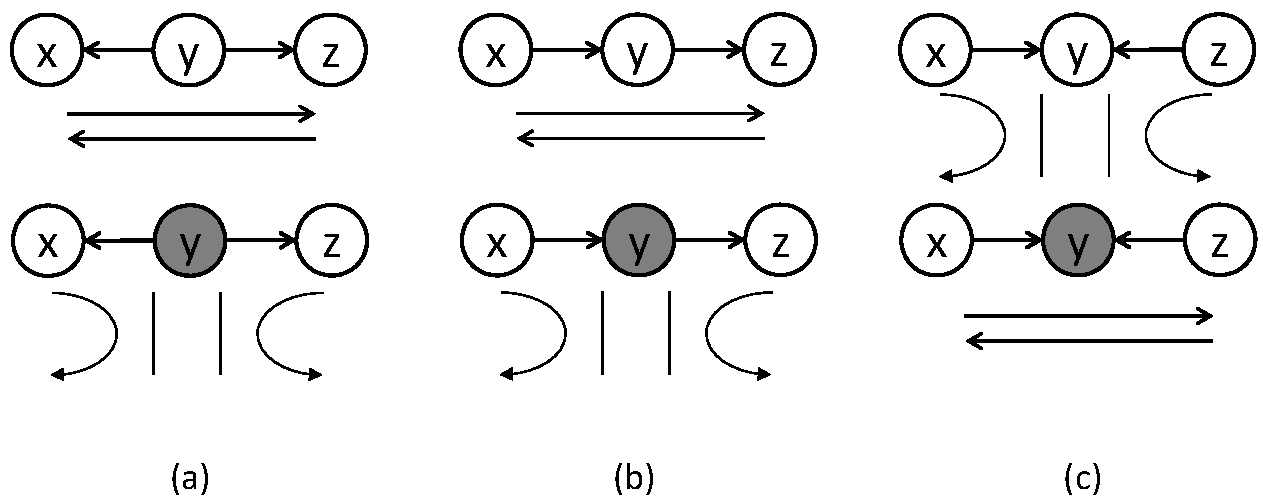
\includegraphics[angle=270,width=\textwidth]{conditional_indepedence.pdf} 

  \caption{不同情况下的独立性质示意图} \label{fig:depedence}
\end{figure}
通过有向图模型可以很容易写出联合分布,但是由其定义的节点之间的独立关系却不显然的。这里仅讨论三种简单的拓扑,其他任何复杂的拓扑形式的独立性质都可以从这几种基础形式根据一定的规则得到。

考虑图\ref{fig:depedence}(a)中尾对尾情况,在未观察到$y$时,$x$和$z$不是独立的:
\begin{equation}
p(x,z) = \int p(x,y,z) dy = \int p(x)p(y,z|x) dy  = p(x)p(z|x) \neq p(x)p(z) 
\end{equation}
如图\ref{fig:depedence}(a)上图所示,可以认为未观察到y时,没有阻止x到z的联系,所以x和z是不独立的。

而在观察到$y$时,$x$和$z$则是条件独立的:
\begin{equation}
\begin{split}
&p(x,z|y)p(y) = p(x)p(y|x)p(z|y)\\
&p(x,z|y) = p(x|y)p(z|y)
\end{split} 
\end{equation}
如图\ref{fig:depedence}(a)下图,可以认为此时由于y被观察到,阻止了x到z的联系。

对于另外两种情况也是类似的。考虑图\ref{fig:depedence}(b)头对尾的情况,易得:
\begin{equation}
\begin{split}
&p(x,z) \neq p(x)p(z)\\
&p(x,z|y) = p(x|y)p(z|y)
\end{split} 
\end{equation}

考虑图\ref{fig:depedence}(c)头对头的情况,易得:
\begin{equation}
\begin{split}
&p(x,z) = p(x)p(z)\\
&p(x,z|y) \neq p(x|y)p(z|y)
\end{split} 
\end{equation}

注意,头对头时的情况和上面两种不一样,在未观察到y的时候,x和z是独立的,然而在观察到y的时候,x和z却不是条件独立的,这一现象称为explaining away。更加详细的讨论可参考\cite{bishop2006pattern}。

另外,对于任意两个节点集,对于他们的(条件)独立性质有一个称为d-划分的定理,利用这个定理,对于任何拓扑,都能够得到其节点间的独立关系。
\subparagraph{D-分割}
对于$A$、$B$和$C$三个互不相交的节点集,考察$A$中任意节点到$B$中任意节点之间的路径。如果某一条路径满足下面的情况之一,则称该路径是被阻塞的:
\begin{itemize}
   \item 路径中存在的尾对尾的节点或者头对尾的节点均在$C$集合中。
   \item 路径中存在的所有头对头节点以及它们的子孙节点均不在$C$集合中。
\end{itemize}
如果$A$到$B$的所有路径都是阻塞的,则称A集合和B集合是被$C$集合d-分割的。

\subparagraph{马尔科夫blanket}
对于有向图模型中某一节点,由该节点的父节点、子节点以及同子父节点(和该节点拥有相同子节点的节点)构成的集合称为的该节点马尔科夫blanket。根据上面介绍的定理,可以很容易推导出,当观察到某节点的马尔科夫blanket时,该节点与其他所有节点是条件独立的。
\begin{figure}
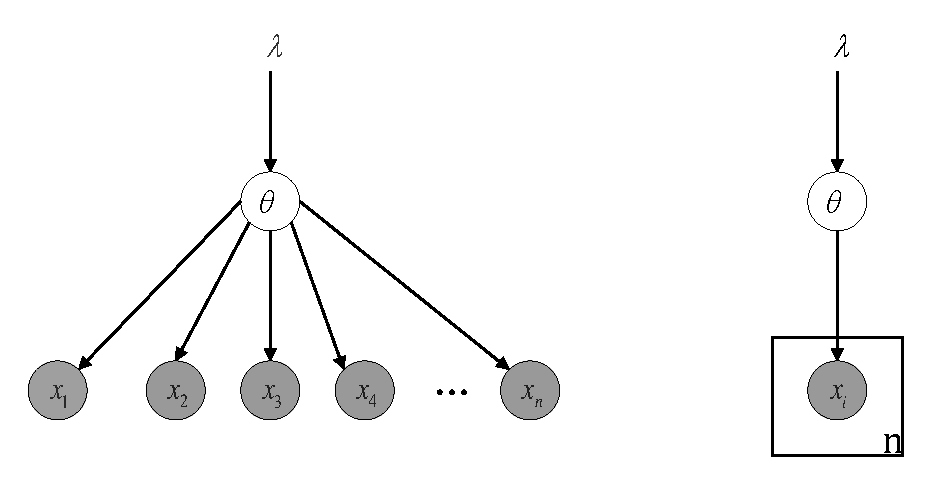
\includegraphics[width=\textwidth]{plate_notation.pdf} 
  \caption{左图:多个独立同分布的节点。右图:使用堆叠记法进行简化} \label{fig:plate_notation}
\end{figure}
\subparagraph{堆叠记法}
对于多个独立同分布变量,如图\ref{fig:plate_notation}左所示,如果一一表示出来,会非常繁琐,所以一般将其简化为用单个节点和带有个数标记的方框来表示,如图\ref{fig:plate_notation}右所示。

\subsection{无向图模型}
本文主要使用有向图模型来进行建模,然而有向图的一些推断算法需要先将其转换为无向图的形式,这一转换非常简单,只要将边上的箭头去除,并将所有的同子父节点相连即可。

D$V_i$、$V_j$和$V_k$是三个互不相交的节点集,如果从$V_i$中的某一节点到$V_k$中的某一节点必然要经过$V_j$,则称$V_j$是一个{分割集}。对于无向图模型,其中任意两个节点集在其分割集上是条件独立的,即:
\begin{equation}
p({\bm x}_{V_i},{\bm x}_{V_k}|{\bm x}_{V_j}) = p({\bm x}_{V_i}|{\bm x}_{V_j})p({\bm x}_{V_k}|{\bm x}_{V_j})
\end{equation}
这个性质称为无向图模型的全局马尔科夫性,因此无向图模型又称马尔科夫随机场。

注意,当一个有向图转化为无向图表示后,此时的无向图形式仍能表征出的独立性是原来的有向图中也有的。但是反之则不然,一些有向图中的独立性,在无向图里无法表现。这说明无向图和有向图并不等价。但是,这不意味着无向图的表示空间就是有向图的表示空间的子集,因为也存在一些无向图是无法用有向图表示的。考虑一个最简单的三个节点全连接的无向图,根据之前的讨论易知,只有9种有向图对应的无向图是这种形式,而这9种有向图必然存在某两个节点在观察到或者未观察到另一个节点时是条件独立的。而这个无向图却可以表示出另一种模型:这三个节点两两之间,无论在什么情况都是不独立的。故无向图的表示空间不是有向图的表示空间的子集。

对于无向图模型,其联合概率的分解形式并不像有向图那么直接。令$C$表示一个无向图模型$G$中的所有全联通子图组成的集合,这里定义一组全联通子图上的函数$\psi_c(.)$,如果关于随机变量$V$的联合分布可以分解为如下形式:
\begin{equation}
p({\bm x}_{V}) \propto \prod_{c \in C} \psi_c({\bm x}_c)
\end{equation}
则这组随机变量的联合分布对应的无向图表示$G$是具有全局马尔科夫性质的。反之,如果对于所有的x满足其概率p(x)是严格正的,则其联合分布对应的马尔科夫随机场一定可以按上式分解。这个理论称为Hammersley-Clifford定理。具体的证明以及进一步讨论可参考\cite{Besag:74,Clifford:90}。


\subparagraph{pairwise马尔科夫随机场}
考虑一种不存在环的无向图,或称为树状的无向图模型。如果一个有向图其对应的无向图是树状的,则其有向图形式和无向图形式表征的独立性是一致。对于树状的模型,任何一个单一的节点$v$都是一个分割集,它将随机变量分为几个子树(如图\ref{fig:belief_propagation}左),这些子树间的节点在观察到v时是条件独立的。这种独立性对于其对应的有向图也是一样的情况。

对于pairwise马尔科夫随机场,其所有的全联通子图集合即由其所有的节点和所有的边组成的集合。故其分解形式为:
\begin{equation}
p({\bm x}_{V}) \propto \prod_{(i,j) \in E} {\psi_{ij}(x_i,x_j)} \prod_{i \in V} \psi_{i}(x_i)
\end{equation}

许多重要的序列模型,如隐马尔科夫模型、状态空间模型等,其对应的无向图模型都是pairwise马尔科夫随机场。

\subsection{置信传播算法}
\begin{figure}
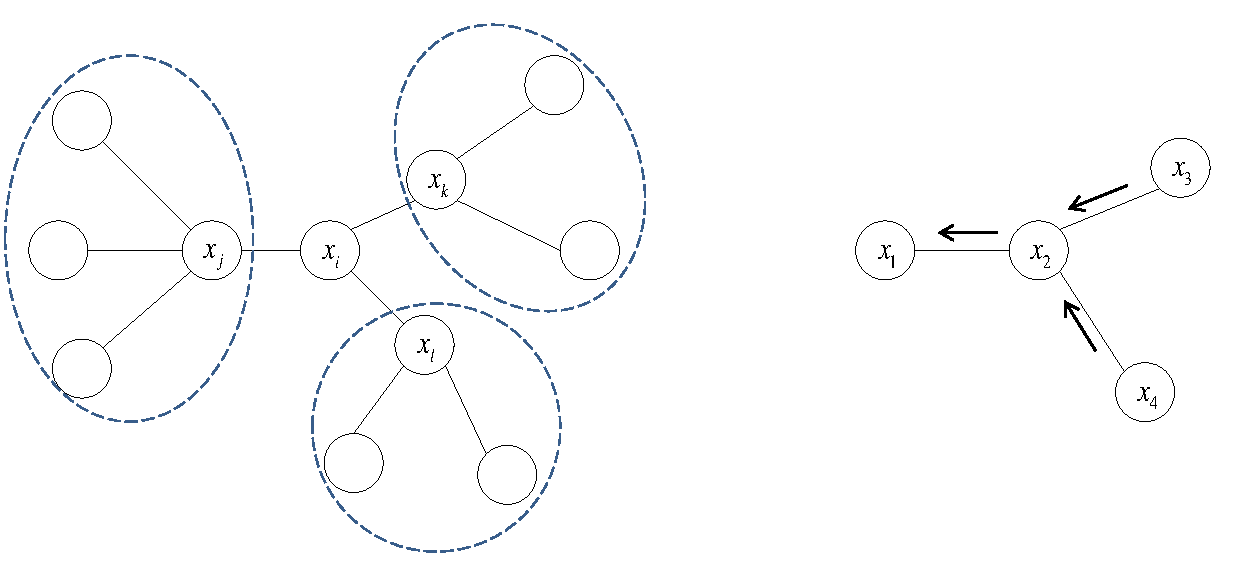
\includegraphics[width=\textwidth]{belief_propagation.pdf} 

  \caption{左图:$x_i$将无向图分割为三个子树  右图:简单的消息传播示意图}\label{fig:belief_propagation}
\end{figure}
在大部分应用中,随机变量的联合空间都会很大,以至于推断任务变得很难。比如,考虑一个含有N个节点的图模型,每个节点的取值空间是一个含有K个值的离散空间,则联合状态空间的大小为$K^N$,如果需要计算某个变量在观察值下的条件边缘概率,对于含有K个值的图,则需要求$K_{N-1}$项的和。

对于树形的图模型,可以通过递归的进行局部计算,从而有效的降低算法的复杂度。由于树状模型中任何一个节点都是分割集,他将原模型划分为几个树形的子图模型。下面介绍一种叫做置信传播的算法\cite{Shafer:90},可以通过将子图计算的结果联合起来得到全图的计算结果。


考虑图\ref{fig:belief_propagation}右的情况,关于${\bm x}$的联合概率分布可以分解成:
\begin{equation}
p({\bm x}) \propto \psi_{12}(x_1,x_2)\psi_{23}(x_2,x_3)\psi_{24}(x_2,x_4)\psi_{1}(x_1)\psi_{2}(x_2)\psi_{3}(x_3)\psi_{4}(x_4)
\end{equation}

求边缘概率分布$p(x_1)$时,可将不同的积分项分离:
\begin{equation}
p(x_1) \propto \psi_{1}(x_1) \int_{x_2}{\psi_{12}(x_1,x_2)\psi_{2}(x_2) \underbrace{\left[ \int_{x_3}\psi_{23}(x_2,x_3) \psi_{3}(x_3)d {x_3} \right]}_{m_{32}(x_2)}  \underbrace{\left[ \int_{x_4}{\psi_{24}(x_2,x_4)\psi_{4}(x_4)} d {x_4} \right]}_{m_{42}(x_2)} } d {x_2} \label{eq:bp_example_raw}
\end{equation}

这里,定义一个称为{消息}的变量${m_{ji}(x_i)}$来表示上式中对$x_j$进行积分且结果是关于$x_i$的函数的项,这样上式就变为了:
\begin{equation}
{m_{21}(x_1)} \propto \int_{x_2}{\psi_{12}(x_1,x_2)\psi_{2}(x_2) {m_{32}(x_2)} {m_{42}(x_2)} } d {x_2} \label{eq:bp_example_m}
\end{equation}

如果考虑更一般的情况,假设图中存在一组观察节点${\bm y}$,不失一般性,假设$y_i$和$x_i$相连,则可以将式\eqref{eq:bp_example_m}推广到一般的情况:
\begin{equation}
{m_{ji}(x_i)} = \int_{x_j}\left({\psi_{ij}(x_i,x_j)\psi_{i}(x_i,y_i) \prod_{k \in \Gamma(j)\backslash i}{m_{kj}(x_j)} }\right) d {x_j} \label{eq:massage_passing_general}
\end{equation}

其中$\Gamma(j)$表示j的相邻节点集合。可以将这个公式看做是一个消息节点间传递的过程:对于节点j,收集其收到的消息,然后将其加工再传给i节点。

另外,叶子节点上的初始消息为:
\begin{equation}
{m_{.i}(x_i)} = 1 \label{eq:massage_passing_leaf}
\end{equation}

利用上面的公式,从叶子节点递推的计算出所有节点之间传播的消息后,就可以得到任意需要的边缘概率分布:
\begin{equation}
p(x_i|{\bm y}) = \frac{1}{Z} \psi_i(x_i,y_i)\prod_{j \in \Gamma(i)}{m_{ji}}
\end{equation}
其中:
\begin{equation}
Z =  \int_{x_i} {\psi_i(x_i,y_i)\prod_{j \in \Gamma(i)}{m_{ji}}} d {x_i}
\end{equation}

一些常用的序列模型中的经典算法如隐马尔科夫模型中的前向后向算法\cite{rabiner1989tutorial},状态空间模型中的卡尔曼滤波算法等都是置信传播算法的特殊形式。对于非树形的图模型,上面的算法不再成立,需要使用loopy置信传播算法,具体细节可参考\cite{pearl1988probabilistic}。

\subsection{有限混合模型}\label{sec:finite_mix}
本文在\ref{sec:exp_family}节介绍了指数函数族,用于表征观察数据的分布情况。然而有时候数据并不是简单的单一分布,而是服从多重模态(mult-modes)分布。此时,通常用有限混合模型\cite{mclachlan2004finite}来建模数据。一个含有K个混合成分的模型的如下:
\begin{equation}
p(x |\pi,\theta_1,...,\theta_K) = \sum_{k=1}^K{\pi_kf(x|\theta_k)} \label{eq:mix_dis}
\end{equation}
其中每个混合成分对应着一个概率密度函数$f(x|\theta_k)$,这里统一记为$F(\theta_k)$。

对于混合模型,每个观察$x_i$的生成过程是:首先根据一个参数为$\pi$的K维的多项分布选择一个成分k,然后从第k个成分对应的概率密度函数中生成$x_i$:
\begin{equation}
\begin{split}
& z_i \sim \pi\\
& x_i \sim F(\theta_{z_i}) \label{eq:aux_finite_mix_g}
\end{split}
\end{equation}
$z_i$是用来表示$x_i$对应隐成分的指示变量,即$z_i = k $表示$x_i$是从第$k$个成分的概率密度中采样的。

在大部分应用中,$f(x|\theta_k)$都是指数函数族,比如当其是高斯分布时,对应的混合模型就是常用的混合高斯模型(GMM)。

对于这个模型,可以用最大化观察值联合似然的方法来估计模型的参数值,也可以用贝叶斯方法计算参数的后验概率分布。当使用贝叶斯方法时,需要为参数加上一个共轭先验分布:
\begin{equation}
\begin{split}
& \theta_k \sim G_0(\lambda) , \quad k = 1,...,K\\
& \pi \sim Dir(\frac{\alpha}{K},...,\frac{\alpha}{K})\\
\end{split} \label{eq:aux_finite_mix_p}
\end{equation}

这里还可以用另一种方法来表示上述的贝叶斯混合模型\footnote{理解这种表示方法对于理解Dirichlet过程非常重要。}。考虑一个在聚类参数空间${\bm \Theta}$(即$\theta$所在的空间,而不是观察值的空间)上的离散分布$G$:
\begin{equation}
\begin{split}
& \theta_k \sim G_0(\lambda), \quad k = 1,...,K\\
& \pi \sim Dir(\frac{\alpha}{K},...,\frac{\alpha}{K})\\
& G(\theta) = \sum_{k=1}^K\pi_k\delta_{\theta_k}\\
\end{split} \label{eq:finite_mix_p}
\end{equation}
其中$\delta_{\theta_k}$表示一个关于$\theta$的函数,其在$\theta_k$处取1而在其他点处为0的函数。

然后,按照如下过程生成$x_i$:
\begin{equation}
\begin{split}
& \phi_i \sim G\\
& x_i \sim F(\phi_i) \label{eq:finite_mix_g}
\end{split}
\end{equation}
这个生成过程和上面使用只是变量z的生成过程是一致的。图\ref{fig:finite_mix}给出了这两种不同的表示法对应的图模型。

需要注意的是,有限混合模型中的混合数是确定的。然而,在实际问题中,往往不知道成分的个数,从而需要用到一些模型选择的方法来选择合适的K。后文将讨论一种称为Dirichlet过程混合的模型,可以有效地解决这个问题。
\begin{figure}
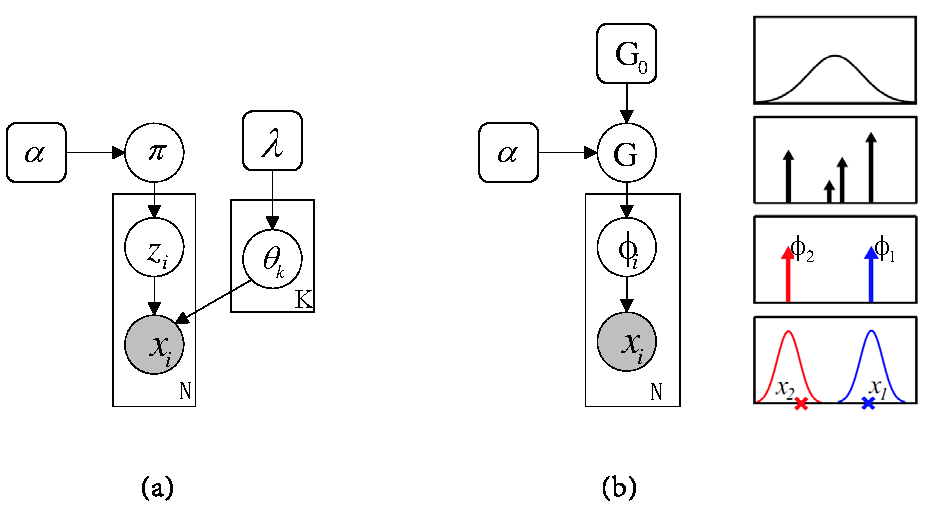
\includegraphics[angle=270,width=\textwidth]{finite_mix.pdf} 
  \caption{有限混合模型的图模型表示} \label{fig:finite_mix}
\end{figure}

\subsection{隐马尔科夫模型}\label{subsec:hmm}
混合模型假设样本是可交换顺序的,但是在一些问题中,样本却是有顺序相关性的。比如在对语音序列建模中,由于语音信号是连续变化的,相邻时间片的样本是相关的,故不能直接使用混合模型进行建模。这里考虑对混合模型进行时间上的扩展。假设对于$t$时刻的样本,其成分变量$z_t$并不是服从从参数为$\pi$的同一个离散分布,而是服从一个和前$n$个时刻相关的离散分布,即:
\begin{equation}
z_t \sim \pi_{z_{t-n},...z_{t-1}}
\end{equation}
注意,在这个模型里,$\pi$的个数是$K^n$个,其中$z_t \in \{1,...,K\}$。

这一模型称为n阶隐马尔科夫模型(hidden Markov models,HMM)\cite{rabiner1989tutorial}。其中经常使用的是$1$阶HMM,即$z_t$服从一个和$z_{t-1}$相关的离散分布。隐马尔科夫模型在对各种序列建模的任务中应用广泛,如生物信息挖掘中对基因序列的建模任务\cite{haussler1996generalized},自然语言处理中的分词、标注、实体名提取等任务\cite{zhou2002named},语音中对音素的建模任务。但是,隐马尔科夫模型中的$z_t$服从一个$K$维的离散分布,这使得在实际应用中,需要用模型选择的方法来确定一个最优的$K$,后文将讨论对其的改进方法。

\subsection{隐狄利克雷分配}\label{subsec:lda}
\begin{figure}
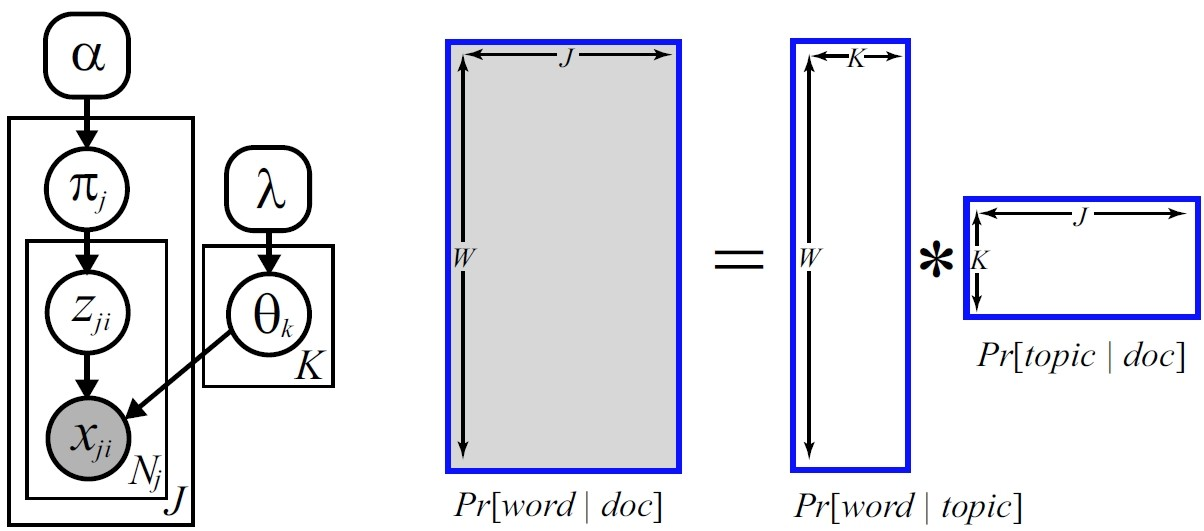
\includegraphics[width=\textwidth]{lda.jpg} 
\caption{LDA的图模型表示}\label{fig:lda}
\end{figure}
上面考虑的都是单组数据的问题,然而,许多任务需要处理多组数据,这些数据的生成过程往往是相关的,但是并不完全相同。如果单独为每组数据建模,就无法利用到他们之间的关联性,而如果将其看做是单一的一组可交换的数据,又会丢失掉他们天生的判别信息。比如在文本语料中,有多个文档,如果为每个文档建立单独的混合模型,则没有建模文档之间的相关性,如果把所有文档看做是一个可交换性的文档建立一个混合模型,则丢失了文档之间的判别信息。所以可以考虑建立一种层次模型,通过在不同的组之间共享参数来建模相关性,而用另一些参数来控制这组共享参数的权重从而表示他们的区分性。

隐狄利克雷分配(latent Dirichlet allocation,LDA)\cite{blei2003latent}就是利用这种思路,通过对混合模型进行层次扩展得到的一种用来建模多组相关数据的层次贝叶斯模型。考虑一个数据集,含有J组数据${\bm x} = ({\bm x}_1,...,{\bm x}_J)$,其中第j组数据集中有$N_j$个样本${\bm x}_j = (x_{j1},...,x_{jN_j})$。整个数据集表示为

在利用LDA建模时,假设每组数据内的样本是可交换的,并且独立同分布于一个含有K个成分的混合模型,而各组的K个成分是共享的。用${\{\theta_k\}}_{k=1}^K$表示混合成分的参数,用${\bm \pi}_j$表示第$j$组数据的混合权重,则对于第j组数据有:
\begin{equation}
p(x_{ji}|{\bm \pi}_j,\theta_1,...,\theta_K) = \sum_{k=1}^K\pi_{jk}f(x_{ji}|\theta_k),\pi_j \in \Pi_{K-1}
\end{equation}
可以看出,LDA使用组间共享参数$\theta$用来建模样本间的相关性,使用组内自有的${\bm \pi}_j$用来建模各组的差异。和贝叶斯混合模型一样,需要为参数${\bm \pi}$加上一个先验\footnote{如果模型不加这个先验,得到的是概率隐语义分析模型(PLSA)}。LDA假设不同组之间是具有交换性的,根据De Finetti定理\cite{de1931funzione},这组权重参数可以看做是从同一个先验分布中独立采样的,所以这里加入一个离散分布的共轭先验,即Dirichlet分布:
\begin{equation}
{\bm \pi}_j \sim Dir(\alpha) j = 1,...J
\end{equation}
另外,也需要为成分参数$\theta$加上一个先验$G_0(\lambda)$,此时得到的LDA模型对应的图模型表示见图\ref{fig:lda}。

如果用混合模型的另一种表示法(式\eqref{eq:finite_mix_p}和式\eqref{eq:finite_mix_g})来表示每组数据的混合模型,则可以得到LDA的另一种等价生成过程:
\begin{equation}
\begin{split}
& \pi_j \sim Dir(\frac{\alpha}{K},...,\frac{\alpha}{K})\\
& \theta_k \sim G_0(\lambda), k = 1,...,K\\
& G_j(\theta) = \sum_{k=1}^K\pi_{jk}\delta_{\theta_k}\\
& \phi_{ji} \sim G\\
& x_{ji} \sim F(\phi_{ji}) 
\end{split} \label{eq:LDA_alt}
\end{equation}

LDA最早是被用于文本分析,它可以从文档中无监督的学习到多个主题(即单词的分布),以及得到文档在主题维度上的表示。对于离散数据,LDA可以得到一个低秩的矩阵分解近似解。然而,只要选择合适的$F(\theta)$,LDA也可以用来建模连续数据。其相关的推断算法可以参考文献\cite{blei2003latent,heinrich2005parameter}。

和有限混合模型和隐马尔科夫模型类似,LDA同样需要手动设定混合成分个数,后文中将介绍一种LDA的非参数模型扩展,可以自动的从数据中推断出混合成分的个数。


\subsection{概率模型间关系}

\begin{figure}
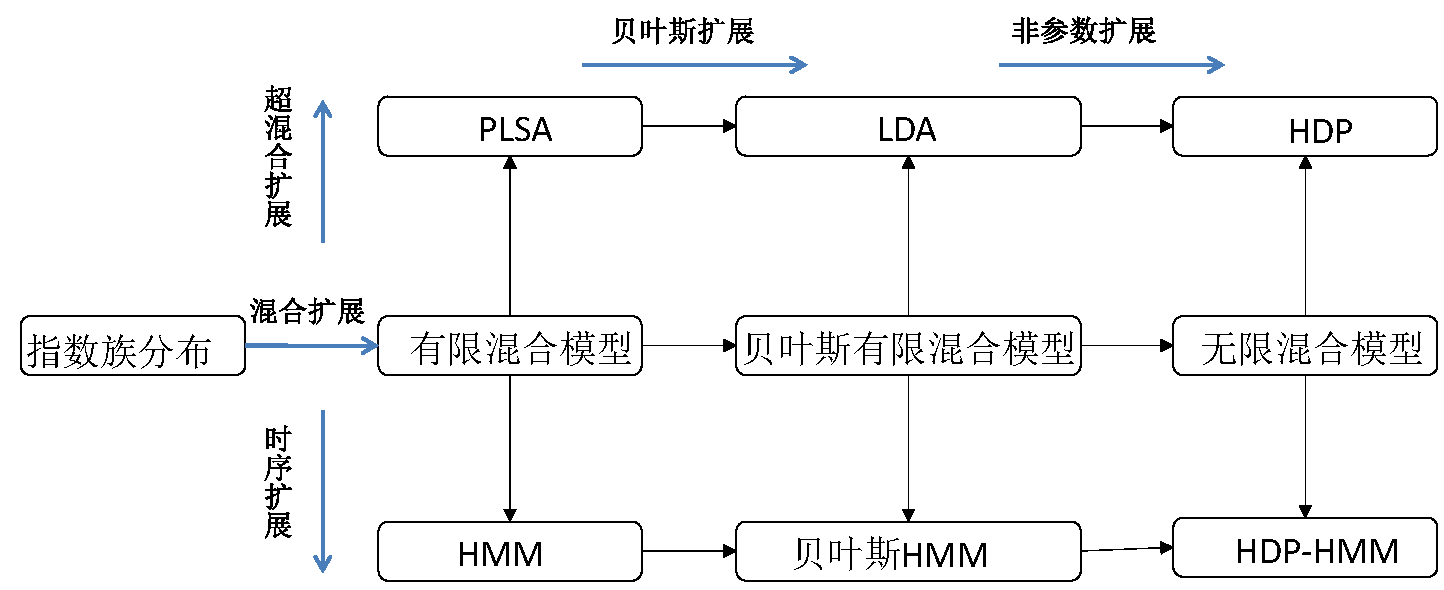
\includegraphics[angle=270,width=\textwidth]{model_relation.pdf} 
\caption{常用的概率模型之间关系}\label{fig:model_relation}
\end{figure}


本章介绍的几种概率模型,通过对基本的指数族分布进行混合、超混合和时序扩展,得到了一系列具有不同性质的模型。其中,混合模型用于建模多成分混合的数据,超混合模型用于建模共享多个成分的多组数据,时序模型用来建模在时间上相关的数据。进一步,通过贝叶斯扩展,可以得到这些模型对应的贝叶斯模型。这些模型的参数个数是固定的,统称为参数模型。对于某个模型,其概率图拓扑和概率函数已经确定,此时其模型的复杂度由参数的个数决定。然而,如果复杂度与问题不一致,会导致过拟合或者欠拟合的问题,这就需要通过手工调整参数个数,来选择复杂度合适的模型,这一过程也称为模型选择。在下一章将研究的Dirichlet过程,可以用来对这些模型进行进一步扩展,使得其变为非参数贝叶斯模型。这类非参数模型的参数个数会根据数据的分布而自适应的变化,从而可以为研究模型选择的问题提供了新的方法。图\ref{fig:model_relation}给出了这些模型之间的关系。



\section{Gibbs采样}
对于一个概率分布$p(x)$,$x \in \chi$,如果能设计一个概率分布$q(.|.)$,使得从初始状态$x^{(0)} \in \chi$出发,在$t>0$时按照该分布不断采样,最终得到的$x$的经验分布和$p(x)$是一致的:
\begin{equation}
x^{(t)}\sim q(x|x^{(t-1)})    t =1,2,...
\end{equation}
那么只需要迭代足够多次,即可以得到真实分布的估计。

这个方法称为马尔科夫链蒙特卡洛方法(Markov chain Monte Carlo,MCMC)\cite{gilks2005markov},其关键在于找到一个使上述假设成立的$q$。Metropolis-Hastings算法提供了一种通用的框架来构造$q$,具体细节可参考\cite{chib1995understanding}。

这里介绍一种特殊的MCMC,称为Gibbs采样。假设样本空间是N维的,对于待采样的N个变量$x=\{x_1,...,x_N\}$,如果每个变量在给定其他N-1个变量时的条件概率都是可以计算的,那么在第$t$次迭代时进行如下的采样:
\begin{equation}
\begin{aligned}
x_i^{(t)}\sim & p(x_i|x_j^{(t-1)},j \neq i)    	& i = i(t)\\
x_j^{(t)}\sim & x_j^{(t-1)}						& j \neq i(t)
\end{aligned}
\end{equation}
即对第$i(t)$维变量进行重新采样,而保持其他维的变量不变。

当这个过程迭代进行无限次时,$x_{(t)}$可以收敛到$p(x)$的真实采样。

\subsection{有限混合模型的Gibbs采样}
这里用有限混合模型的推断作为例子来展示Gibbs采样的过程。在有限模型(图\ref{fig:finite_mix})中,观察值为$x= {\{x_i\}}_{i=1}^N$,需要推断的变量为成分指示变量$z= {\{z_i\}}_{i=1}^N$、混合参数$\pi$、成分参数$\theta= {\{\theta_k\}}_{k=1}^K$。这里主要是展示Gibbs采样,不考虑模型的参数的学习问题,假定其为固定值。

根据Gibbs采样算法,需要求得每个变量在其他变量已知时的条件概率。首先考虑z,对于$z_i$,根据概率模型中的概率依赖关系,可以得到:
\begin{equation}
\begin{aligned}
p(z_i=k|z^{-i},x,\pi,\theta_1,...,\theta_K) & \sim p(z_i=k|\pi)p(x_i|z_i,\theta_1,...\theta_K)\\
											& = \pi_kf(x_i|\theta_k)
\end{aligned}
\end{equation}
其中$z^{-i}$表示$z$中除去$z_i$的其他变量。

下面给出详细的解释。首先,有
\begin{equation}
\begin{aligned}
p(z_i=k|z^{-i},x,\pi,\theta_1,...,\theta_K) &=  \frac{p(z_i=k,x_i|z^{-i},x^{-i},\pi,\theta_1,...,\theta_K)}{\sum_{k=1}^{K}p(z_i=k,x_i|z^{-i},x^{-i},\pi,\theta_1,...,\theta_K)}\\
											&\propto p(z_i=k,x_i|z^{-i},x^{-i},\pi,\theta_1,...,\theta_K)\\
											&\propto p(z_i=k|z^{-i},x^{-i},\pi,\theta_1,...,\theta_K)p(x_i|z_i,z^{-i},x^{-i},\pi,\theta_1,...,\theta_K)
\end{aligned}
\end{equation}

对于右边第一项,当观察到$\pi$时,$z_i$和$z^{-i}$,$\theta^{-{z_i}}$,$x^{-i}$条件独立。当未观察到$x_i$时,$z_i$和$\theta_{z_i}$独立,从而第一项可以写为$p(z_i=k|\pi)$。对于右边第二项,当观察到$z_i$和$\theta_{z_i}$时,$x_i$和其余变量条件独立,故可以写为$p(x_i|z_i,\theta_{z_i})$。

对于$\pi$和$\theta= {\{\theta_k\}}_{k=1}^K$,可知他们在观察到z的情况下是条件独立的,结合模型中其他的独立性质,有:
\begin{equation}
p(\pi,\theta_1,...,\theta_K|z,x) = p(\pi|z)\prod_{k=1}^K{p(\theta_k|\{x_i|z_i=k\})}
\end{equation}
其中每一项利用贝叶斯条件法则即可求得。

\subsection{Collapsed Gibbs采样}
Gibbs采样需要迭代较多次才能收敛,根据Rao–Blackwellized理论,如果可以用解析的方法积分掉某些变量以减小采样空间,则采样的过程可以更快的收敛。这种方法通常称为Rao–Blackwellized Gibbs采样或collapsed Gibbs采样\cite{casella1996rao}。

仍然考虑有限混合模型的采样问题,由于为$\pi$增加的是共轭先验,故考虑将$\pi$解析的积分掉。则此时待采样变量减少为$z= {\{z_i\}}_{i=1}^N$和$\theta= {\{\theta_k\}}_{k=1}^K$。根据概率图模型中的独立关系,有:
\begin{equation}
p(z_i=k|z^{-i},x,\theta_1,...,\theta_K) \propto p(z_i=k|z^{-i})p(x_i|z_i,\theta_1,...\theta_K) \label{eq:finite_collapsed_gibbs_pi}
\end{equation}

如果$\theta$的先验$G_0(\lambda)$是共轭先验,则可以将$\theta$也解析的积分掉。此时的采样空间进一步变小,待采样的变量仅为$z= {\{z_i\}}_{i=1}^N$,根据概率图模型中的独立关系,有:
\begin{equation}
p(z_i=k|z^{-i},x,\theta_1,...,\theta_K) \propto p(z_i=k|z^{-i})p(x_i|\{x_j|z_j=k,j \neq i\}) \label{eq:finite_collapsed_gibbs_pi_theta}
\end{equation}